% WisdomFusion#gmail.com
% 20120602
%
\documentclass[12pt,a4paper,twoside]{ctexart}
%-------------------- 引用宏包--------------------
\usepackage[landscape,textheight=190mm,textwidth=145mm,left=20mm,right=20mm,top=20mm,bottom=15mm]{geometry}
\usepackage{graphicx}
\usepackage{fontspec}
\usepackage{fancybox}
\usepackage{colortbl}
\usepackage{fancyhdr}
\usepackage[CJKbookmarks,colorlinks,bookmarksnumbered=true,pdfstartview=FitH,linkcolor=black]{hyperref}
\usepackage{longtable,tabularx,booktabs}          % 自动换行用 tabularx,自动换页用 longtable,二者兼得用 ltxtable
\usepackage{multicol,multirow}
\usepackage{xcolor}
\usepackage{tcolorbox}
\usepackage{verbatim}
\usepackage{nameref}
\usepackage[perpage]{footmisc}  % 每页重置脚注编号
\usepackage{pifont}
\usepackage{menukeys}
\usepackage{lipsum}
\usepackage{marvosym}
% --------------------设定样式--------------------
\ctexset{
  section/format+=\raggedright
}

\usepackage{listings}
\lstset{
  upquote,
  keepspaces=true,
  columns=spaceflexible,
  numbers=left,
  basicstyle=\ttfamily\small,
  numberstyle=\color{gray}\ttfamily\scriptsize,
  keywordstyle=\color{blue}\ttfamily,
  stringstyle=\color{red}\ttfamily,
  commentstyle=\color{teal}\ttfamily,
  emphstyle=\color{blue}\bfseries,
  backgroundcolor=\color{yellow!5},
  frameround=ftft,
  frame=trBL
}
\setlength\columnsep{20pt}        % multicolumns 栏间距
\setlength{\tabcolsep}{0.5em}     % 水平padding
\renewcommand{\arraystretch}{1.5} % 垂直padding
\renewcommand\thefootnote{\ding{\numexpr171+\value{footnote}}} % 脚注编号
% --------------------设定字体--------------------
%\setmainfont{Times New Roman}   % 缺省字体
\setmainfont{Georgia}   % 缺省字体
\setCJKfamilyfont{song}{SimSun}
\setCJKfamilyfont{hei}{SimHei}
\setCJKfamilyfont{kai}{KaiTi}
\setCJKfamilyfont{fs}{FangSong}
\setCJKfamilyfont{yahei}{Microsoft YaHei}

\renewcommand\contentsname{目\quad{} 录}

%--------------------新建命令--------------------
\newcommand{\cbregex}[1]{\colorbox{orange!18}{\strut #1}}
\newcommand{\cbmatch}[1]{\colorbox{cyan!35}{\strut #1}}
\newcommand{\cbstring}[1]{\colorbox{green!20}{\strut #1}}

\begin{document}

\title{\textbf{正则表达式快速参考手册}}
\author{胡志飞\\<WisdomFusion\textcolor{cyan}{\small [at]}gmail\textcolor{cyan}{\small [dot]}com>}
\date{2012年之旧文重拾于2016年2月26日\\version 0.1.0}

\maketitle{}
\thispagestyle{empty}
\clearpage{}

\begin{multicols}{2}
\tableofcontents
\end{multicols}

\thispagestyle{empty}
\clearpage{}

\setcounter{page}{1}

\section[简介]{简介 \textcolor{lightgray}{\textsc{Introduction}}}
\label{sec:intro}
文字处理无处不在无时不有,日常工作和学习大多数任务都和文字息息相关,编辑们写文章、整理资料,开发人员编码、处理用户提交的数据或请求接口数据,等等,这些都是以字符和字符串相关的任务,既然如些,掌握一个快速文字处理的方法就变得很有必要。\par
正则表达式,(Regular Expression,在代码中常简写为regex、regexp或RE)~,计算机科学的一个概念。正则表达式使用字符来描述、匹配一系列符合某个句法规则的字符串。在很多文本编辑器里,正则表达式通常被用来检索、替换那些符合某个模式的文本。许多程序设计语言都支持利用正则表达式进行字符串操作。例如,在Perl\footnote{\href{https://www.perl.org/}{Perl}被称为“实用报表提取语言”(Practical Extraction and Report Language)~,正则表达式特性的推动者,文本处理非常方便。}中就内建了一个功能强大的正则表达式引擎。正则表达式这个概念最初是由Unix中的工具软件(例如sed\footnote{\href{http://www.gnu.org/software/sed/manual/sed.html}{sed}是一种UNIX/Linux平台下的轻量级流编辑器,日常一般用于处理文本文件。}和grep\footnote{grep,global search regular expression and print out the line,是一种强大的文本搜索工具,它能使用正则表达式搜索文本,并把匹配的行打印出来。})普及开的。\par
需要注意的是,用什么工具,用什么编辑语言,正则表达式的语法有些差别,特性的支持也参差不齐,称之为正则表达式“流派”(第\ref{sec:flavor}部分详述),所以要单独参考工具和编程语言本身的文档才行。本文档旨在给大家一个通用的、概括的正则表达式宏观印象,辅以实例和应用案例,同时针对个别常用但又不易理解的特性,给大家作详细说明和总结,抛砖引玉。\par
期望本文档能给大家一个快速的参考,快速的掌握正则表达式这个棒棒哒效率工具,让大家平时工作学习中更加得心应手!\Smiley{} \par

\begin{tcolorbox}[colback=yellow!5,colframe=red!80!black,title=\textbf{说明}]
  我对排版及专业出版知之甚微,只是在平时笔记和文档时,哪怕是自己写的太乱的话也不乐意翻看,印象笔记里的东东又过于零碎,故把旧文完善并整排\footnote{本文档2012年编写,现整拾,并加以完善。目前觉得Markdown, \href{http://orgmode.org/}{org-mode}适用于文本文档的快速编写,而Adobe InDesign和LaTeX适合更专业的文档和书籍的图文混排及设计。}。然而,专业领域知识因涉猎过多而不精,难保周全和准确,但只要在自己知识圈内,我会劲力完成尽可能规范和可靠的文档呈现给大家,并不断完善更新,请批评指正,共同提高。
\end{tcolorbox}

\section[基本语法]{基本语法 \textcolor{lightgray}{\textsc{Basic Syntax}}}
\label{sec:basic-syntax}

语法部分结合了自己的理解和对正则表达式应用的一些心得,分类有不当之处,请指正。因为是总结性的参考文档,所以这里使用“大表哥”形式展示,列出语法的同时,关键语法举了几个栗子加强理解。\par

\begin{center}
  
\begin{longtable}{p{4em}p{8em}p{25em}p{18em}}
  \toprule
  \textbf{特性} & \textbf{语法} & \textbf{描述} & \textbf{举个栗子} \\
  \midrule
  \endfirsthead                 %
  \multicolumn{4}{l}{(续表)} \\
  \toprule
  \textbf{特性} & \textbf{语法} & \textbf{描述} & \textbf{举个栗子} \\
  \midrule
  \endhead                      %
  \multicolumn{4}{c}{To be continued\ldots} \\[2ex]
  \endfoot                      %
  \bottomrule
  \endlastfoot                  %
  %--------------------
  字符 & 除[\textbackslash{}\^{}\$.|?*+()以外的任意字符 & 除了[\textbackslash{}\^{}\$.|?*+()以外的任意字符,\{和\}也是文字文本,除了下面说到的成对出现的量词语法,如\{n\}和\{m,n\}等。& \cbregex{a}匹配\cbstring{about}中的\cbmatch{a} \\
  & 字符转义 & \cbregex{\textbackslash{}t}, \cbregex{\textbackslash{}?}, \cbregex{\textbackslash{}*}, \cbregex{\textbackslash{}+}, \cbregex{\textbackslash{}.}, \cbregex{\textbackslash{}|}, \cbregex{\textbackslash{}\{}, \cbregex{\textbackslash{}\}}, \cbregex{\textbackslash\textbackslash}, \cbregex{\textbackslash{}[}, \cbregex{\textbackslash{}]}, \cbregex{\textbackslash{}(}, \cbregex{\textbackslash{})} & \cbregex{\textbackslash{}+}匹配\cbmatch{+};\cbregex{\textbackslash{}?\textbackslash{}-}匹配\cbmatch{?-} \\
  & \cbregex{\textbackslash{}n}, \cbregex{\textbackslash{}r} 和 \cbregex{\textbackslash{}t} & Windows文件格式换行符是\textbackslash{}r\textbackslash{}n,UNIX文件格式换行符是\textbackslash{}n,\textbackslash{}t 匹配水平制表符 & \\
  & \cbregex{\textbackslash{}cA}到\cbregex{\textbackslash{}cZ}, \cbregex{\textbackslash{}ca}到\cbregex{\textbackslash{}cz} & \keys{Ctrl + A} 到 \keys{Ctrl + Z},与ASCII字符\cbregex{\textbackslash{}x01}到\cbregex{\textbackslash{}x1A}等价 & \\
  & \cbregex{\textbackslash{}a}, \cbregex{\textbackslash{e}}, \cbregex{\textbackslash{}f}, \cbregex{\textbackslash{}v} & 依次为警报(\textbackslash{}x07)、Esc字符(\textbackslash{}x1B)、进纸符(\textbackslash{}x0C)和垂直制表符(\textbackslash{}x0B) & \\
  & \cbregex{\textbackslash{}Q}\ldots\cbregex{\textbackslash{}E} & 文字文本范围,被包含在\cbregex{\textbackslash{}Q}和\cbregex{\textbackslash{}E}之间的文字,都被视为普通文字,如[\textbackslash{}\^{}\$.|?*+()\{\}也不再用转义了,这个最早是由Perl引入正则表达式的。& \cbregex{\textbackslash{}Q+-*/\textbackslash{}E}匹配的就是\cbmatch{+-*/} \\
  \midrule
  %--------------------
  基本特性 & \cbregex{.}(点) & 匹配除换行符之外的任意字符,有些正则表达式“流派”还支持点是否匹配换行符的开关。& \cbregex{.} 匹配 about 中的任意一个字符 \\
  & \cbregex{|} & 管道,或的关系,匹配|的左侧或右侧的字符串 & \cbregex{abc|def|xyz}匹配\cbmatch{abc}或\cbmatch{def}或\cbmatch{xyz} \\
  \midrule
  %--------------------
  字符类 & \cbregex{[\ldots]} & 匹配字符类中列举的任意一个字符 & \cbregex{[abc]}匹配\cbmatch{a}或\cbmatch{b}或\cbmatch{c}\newline{}\cbregex{[aeiou]}匹配任何一个英文元音字母\newline{}\cbregex{[.!?]}匹配\cbmatch{.}或\cbmatch{!}或\cbmatch{?} \\
  & \cbregex{[\textbackslash{}\^{}\textbackslash{}]]} & 在字符类中,要匹配 \^{}-]\textbackslash{}这几字符,得使用\textbackslash{}转义 & \cbregex{[\textbackslash\^{}\textbackslash{}]]}匹配\cbmatch{\^{}}或\cbmatch{]} \\
  & \cbregex{[\^{}\ldots]} & 排除型字符类,\^{}(脱字符,caret)紧跟 [ 之后,可以把字符类中列举的字符排除匹配范围,也就是所这个字符类将匹配任意一个不在列出字符范围内的字符 & \cbregex{[\^{}a-d]}匹配除了a,b,c,d之外的任意一个字符 \\
  & \cbregex{\textbackslash{}d}, \cbregex{\textbackslash{}w}, \cbregex{\textbackslash{}s} & \cbregex{\textbackslash{}d} 匹配数字,与 \cbregex{[0-9]} 等价;\cbregex{\textbackslash{}w} 匹配任意一个字母或数字或下划线或汉字;\cbregex{\textbackslash{}s} 匹配任意一个空白符 & \cbregex{[\textbackslash{}d\textbackslash{}s]}匹配一个数字或空白符 \\
  & \cbregex{\textbackslash{}D}, \cbregex{\textbackslash{}W}, \cbregex{\textbackslash{}S} & 是 \cbregex{\textbackslash{}d}, \cbregex{\textbackslash{}w} 和 \cbregex{\textbackslash{}s} 的反义字符类。\cbregex{\textbackslash{}D} 匹配任意非数字的字符;\cbregex{\textbackslash{}W} 匹配任意不是字母、数字、下划线、汉字的字符;\cbregex{\textbackslash{}S} 匹配任意不是空白符的字符 & \textbackslash{}D匹配任意非数字的字符 \\
  & \cbregex{[\textbackslash{}b]} & 在字符类中,\cbregex{[\textbackslash{}b]}为\keys{Backspace}退格键字符 & \\
  \midrule
  %--------------------
  POSIX & \cbregex{[:alnum:]} & 匹配所有大小写字母及数字 & 等价于\cbregex{[0-9a-zA-Z]} \\
  & \cbregex{[:alpha:]} & 匹配所有大小写字母 & 等价于\cbregex{[a-zA-Z]} \\
  & \cbregex{[:ascii:]} & 匹配所有ASCII字符,查看完整\href{http://www.asciitable.com/}{ASCII字符列表} & 等价于\cbregex{[\textbackslash{}x01-\textbackslash{}x7F]} \\
  & \cbregex{[:blank:]} & 匹配半角空格和制表符 & 等价于\cbregex{[ \textbackslash{}t]} \\
  & \cbregex{[:cntrl:]} & 匹配所有ASCII 0到31之间的控制符 & 等价于\cbregex{[\textbackslash{}x01-\textbackslash{}x1F]} \\
  & \cbregex{[:digit:]} & 匹配所有数字 & 等价于\cbregex{[0-9]} \\
  & \cbregex{[:graph:]} & 匹配所有可打印的字符 & \\
  & \cbregex{[:lower:]} & 匹配所有小写字母 & 等价于\cbregex{[a-z]} \\
  & \cbregex{[:print:]} & 匹配所有可打印字符和空格 & \\
  & \cbregex{[:punct:]} & 匹配所有标点符号 & \\
  & \cbregex{[:space:]} & 空白字符 & 等价于\cbregex{[\textbackslash{}t\textbackslash{}n\textbackslash{}r\textbackslash{}f\textbackslash{}v]} \\
  & \cbregex{[:upper:]} & 匹配所有大写字母 & 等价于\cbregex{[A-Z]} \\
  & \cbregex{[:word:]} & 字母、数字和下划线 & 等价于\cbregex{[a-zA-Z0-9\_]} \\
  & \cbregex{[:xdigit:]} & 匹配所有十六进制字符 & 等价于\cbregex{[0-9a-fA-F]} \\
  \midrule
  %--------------------
  锚点 & \cbregex{\^{}} & 匹配字符串开始位置或行首位置 & 单行模式下 \cbregex{\^{}.} 在 \cbstring{foo\textbackslash{}nbar} 中匹配 \cbmatch{f};在多行模式下,同时还匹配换行后的 \cbmatch{b} \\
  & \cbregex{\$} & 匹配字符串结尾位置或行尾位置 & \cbregex{.\$} 在 \cbstring{foo\textbackslash{}nbar} 中匹配 \cbmatch{r};在多行模式下,同时还匹配换行符前的 \cbmatch{o} \\
  & \cbregex{\textbackslash{}A} & 字符串开头位置(类似 \^{},但不受处理多行选项的影响)& \cbregex{\textbackslash{}Ae} 在 \cbstring{example} 这个字符串中匹配开头的 \cbmatch{e} \\
  & \cbregex{\textbackslash{}Z} & 字符串结尾位置或行尾位置(不受处理多行选项的影响)& \cbregex{e\textbackslash{}Z} 在 \cbstring{example} 这个字符串中匹配结尾的 \cbmatch{e} \\
  & \cbregex{\textbackslash{}b} & 单词分界位置,单词开头或结尾 & \cbregex{.\textbackslash{}b} 在字符串 \cbstring{abc} 中匹配 \cbmatch{c} \\
  & \cbregex{\textbackslash{}B} & 匹配不是单词开头或结尾的位置 & \cbregex{\textbackslash{}B.\textbackslash{}B} 在字符串 \cbstring{abc} 中匹配 \cbmatch{b} \\
  & \cbregex{\textbackslash{}<} & 单词开头 & \\
  & \cbregex{\textbackslash{}>} & 单词结尾 & \\
  \midrule
  %--------------------
  量词 & \cbregex{?} & 前导字符重复零次或一次,贪婪的\footnote{贪婪模式:当正则表达式中包含能接受重复的限定符时,通常的行为是(在使整个表达式能得到匹配的前提下)匹配尽可能多的字符。考虑这个表达式:\cbregex{a.*b},它将会匹配最长的以\cbmatch{a}开始,以\cbmatch{b}结束的字符串。如果用它来搜索\cbstring{aabab}的话,它会匹配整个字符串\cbmatch{aabab}。这被称为贪婪匹配。}:当正则表达式中包含能接受重复的限定符时,通常的行为是(在使整个表达式能得到匹配的前提下)匹配尽可能多的字符。& \cbregex{abc?} 匹配 \cbmatch{abc} 或 \cbmatch{ab},如果可能,优先匹配前者 \\
  & \cbregex{??} & 前导字符重复零次或一次,非贪婪\footnote{相反,非贪婪,即匹配尽可能少的字符,只要在量词后面加上一个问号?。如\cbregex{a.*?b}匹配最短的,以\cbmatch{a}开始,以\cbmatch{b}结束的字符串。如果把它应用于\cbstring{aabab}的话,它会匹配\cbmatch{aab}(第一到第三个字符)和\cbmatch{ab}(第四到第五个字符)。}:当正则表达式中包含能接受重复的限定符时,通常的行为是(在使整个表达式能得到匹配的前提下)匹配尽可能少的字符。与贪婪相反。& \cbregex{abc??} 匹配 \cbmatch{ab} 或 \cbregex{abc} \\
  & \cbregex{*} & 前导字符重复零次或更多次,贪婪的 & \\
  & \cbregex{*?} & 前导字符重复零次或更多次,非贪婪 & \\
  & \cbregex{+} & 前导字符重复一次或更多次,贪婪的 & \\
  & \cbregex{+?} & 前导字符重复一次或更多次,非贪婪 & \\
  & \cbregex{\{n\}} & 前导字符重复n次 & \\
  & \cbregex{\{n,m\}} & 前导字符重复n到m次,其中$n>=0$,$m>=n$ & \\
  & \cbregex{\{n,\}} & 前导字符重复n次或更多次,其中$n>=0$ & \\
  & \cbregex{\{,m\}} & 前导字符最多重复m次,基中$m>=0$ & \\
  \midrule
  %--------------------
  \multirow{2}{4em}{分组与\newline{}反向引用} & (regex) & 匹配regex,并捕获文本到自动命名的组里 & \cbregex{(abc)\{3\}} 匹配 \cbmatch{abcabcabc} \\
  & (?:regex) & 匹配regex,不捕获匹配的文本,也不给此分组分配组号 & \cbregex{(?:abc)\{3\}} 匹配 \cbmatch{abcabcabc},无分组 \\
  & \textbackslash{}1 到 \textbackslash{}9 & 反向引用,用于重复搜索前面某个分组匹配的文本。例如,\textbackslash{}1代表分组1匹配的文本。有些与此正则表达式流派支持多于9的分组 & \multirow{2}{18em}{\cbregex{(abc|def)=\textbackslash{}1} 匹配 \cbmatch{abc=abc} 或 \cbmatch{def=def},而不是 \cbstring{abc=def} 或 \cbstring{def=abc}} \\
  & \textbackslash{}10 到 \textbackslash{}99 & 反向引用,分组10到99 & \\
  & \textbackslash{}g\{1\} 到 \textbackslash{}g\{99\} & Perl语法中,反向引用语法优化\footnote{如果想实现类似\cbregex{(.)\textbackslash{}1}的效果,若紧跟的字符和分组号相同,如\cbregex{(.)\textbackslash{}111},这样正则表达式引擎就不知所措,如果用\cbregex{\textbackslash{}g\{1\}11}这种语法就不会有歧义,最重要的是这种语法或以用负数分组号倒序选用分组。} & \multirow{2}{18em}{避免出现歧义,同时用负数分组还能倒序引用。} \\
  & \textbackslash{}g\{-1\}, \textbackslash{}g\{-2\}, etc. & 倒数第1个分组,倒数第2个分组,\ldots & \\
  & (?<name>regex) & 命令分组 & 命名分组的最大好处是反向引用时不用再怕弄错分组了。 \\
  & \textbackslash{}k<name> & 反向引用命令分组,Perl中也可以使用\textbackslash{}g\{name\}。 & \\
  & \cbregex{\textbackslash{}\`{}} & 正则表达式匹配部分之前的字符串,Perl语言中也作 \verb=${^PREMATCH}= & \\
  & \cbregex{\textbackslash{}\&} & 正则表达式匹配的部分,Perl语言中也作 \verb=${^MATCH}= & \\
  & \cbregex{\textbackslash{}'} & 正则表达式匹配部分之后的字符串,Perl语言中也作 \verb=${^POSTMATCH}= & \\
\end{longtable}
\end{center}

\section[高级语法]{高级语法 \textcolor{lightgray}{\textsc{Advanced Syntax}}}
\label{sec:adv-syntax}

之所以本文档中称这些正则为“高级语法”,一是有些不常用,二是有些语法不太好理解,故有此一说。

\begin{center}

\begin{longtable}{p{4em}p{9em}p{25em}p{18em}}
  \toprule
  \textbf{特性} & \textbf{语法} & \textbf{描述} & \textbf{举个栗子} \\
  \midrule
  \endfirsthead                 %
  \multicolumn{4}{l}{(续表)} \\
  \toprule
  \textbf{特性} & \textbf{语法} & \textbf{描述} & \textbf{举个栗子} \\
  \midrule
  \endhead                      %
  \multicolumn{4}{c}{To be continued\ldots} \\[2ex]
  \endfoot                      %
  \bottomrule
  \endlastfoot                  %
  %--------------------
  模式\newline{}修饰符 & \cbregex{(?i)} & 打开忽略大小写模式,之后的模式不分大小写。模式修饰符有 i, s, m, x 四种,分别是忽略大小写(\textbf{I}gnoreCase)~、单行模式(\textbf{S}ingleline)~、多行模式(\textbf{M}ultiline)和注释模式 & \multirow{2}{18em}{\cbregex{(?i)te(?-i)st} 匹配 \cbmatch{TEst},而不匹配 \cbstring{TEST}} \\
  & \cbregex{(?-i)} & 关闭忽略大小写模式,之后的模式不分大小写 & \\
  & \cbregex{(?s)} & 打开单行模式,之后的模式不支持多行 & \multirow{2}{18em}{默认情况下\cbregex{.}是不匹配换行的,打开该模式后,待匹配的字符将为视为“一行”。} \\
  & \cbregex{(?-s)} & 关闭单行模式,之后的模式支持多行 & \\
  & \cbregex{(?m)} & 打开多行模式,之后的模式支持多行 & \\
  & \cbregex{(?-m)} & \cbregex{\^{}} 和 \cbregex{\$} 匹配行首和行尾 & \\
  & \cbregex{(?x)} & 打开宽松和注释模式 & \multirow{2}{18em}{打开该模式后,可以在正则表达式中插和空白和换行,使正则表达式可读性增强。} \\
  & \cbregex{(?-x)} & 关闭宽松和注释模式 & \\
  & \cbregex{(?i-sm)} & 打开i和m模式,关闭s模式 & \multirow{2}{18em}{以上几种模式可以组合使用} \\
  & \cbregex{(?i-sm:regex)} & 在\cbregex{(?i-sm:regex)} 子模式内打开i和m模式,关闭s模式 & \\
  \midrule
  %--------------------
  注释 & (?\#comment) & 注释 & \\
  \midrule
  %--------------------
  零宽断言 & (?=Regex) & 肯定顺序环视(Negative Lookahead)\newline{}子表达式 \underline{能}够匹配 \underline{右侧}文本,含以下三种些类正则被称“\textbf{环视}(Lookaround, Lookahead 和 Lookbehind 统称为 Lookaround)”,也称为“\textbf{零宽断言}”(Zero-Length Assertions) & \cbregex{\textbackslash{}b\textbackslash{}w+(?=ing\textbackslash{}b)},匹配以\cbstring{ing}结尾的单词的前面部分(除了\cbstring{ing}以外的部分) \\
  & (?!Regex) & 否定顺序环视(Positive Lookahead)\newline{}子表达式 \underline{不能}匹配 \underline{右侧}文本 & \cbregex{(?<=\textbackslash{}bre)\textbackslash{}w+\textbackslash{}b}会匹配以\cbstring{re}开头的单词的后半部分(除了\cbstring{re}以外的部分)\newline{}又,\cbregex{(?<=\textbackslash{}s)\textbackslash{}d+(?=\textbackslash{}s)}匹配以空白符间隔的数字(再次强调,不包括这些空白符) \\
  & (?<=regex) & 肯定逆序环视(Positive Lookbehind)\newline{}子表达式 \underline{能}够匹配 \underline{左侧}文本 & \cbregex{\textbackslash{}d\{3\}(?!\textbackslash{}d)}匹配三位数字,而且这三位数字的后面不能是数字 \\
  & (?<!regex) & 否定逆序环视(Negative Lookbehind)\newline{}子表达式 \underline{不能}匹配 \underline{左侧}文本 & \cbregex{(?<![a-z])\textbackslash{}d\{7\}}匹配前面不是小写字母的七位数字\newline{}又,\cbregex{(?<=<(\textbackslash{}w+)>).\*(?=<\textbackslash{}/\textbackslash{}1>)}匹配不包含属性的简单HTML标签内里的内容 \\
  \midrule
  固化分组 & (?>regex) & 贪婪子表达式,也称“\textbf{固化分组}”,使用它可以加快匹配失败的速度,如 \cbstring{Subject} 这个字符串,现用 \cbregex{\^{}\textbackslash{}w:} 对其进行匹配,正则表达式引擎发现 \cbstring{Subject} 不匹配,就会试图匹配 \cbstring{Subjec},一直尝试到 \cbstring{S},发现都不匹配才得出无法匹配的结论。如果使用固化分组 \cbregex{\^{}(?>\textbackslash{}w+):},它会直接试图使用 \cbregex{\textbackslash{}w+} 去匹配 \cbstring{Subjec} 字符串,而不会一一回溯,发现 \cbregex{\textbackslash{}w+} 后面没有 \cbstring{:},立即报告失败。 & 如果字符串中没有第二个 \cbstring{x} 的时候,\cbregex{x(?>\textbackslash{}w+)x} 要比 \cbregex{x\textbackslash{}w+x} 高效得多 \\
\end{longtable}

\end{center}

\section[举些例子吧!]{举些例子吧!~\textcolor{lightgray}{\textsc{Regex Examples}}}
\label{sec:regex-examples}

\begin{description}
\item[Email地址] \hfill \\
  \verb=^[a-zA-Z0-9_.+-]+@[a-zA-Z0-9-]+\.[a-zA-Z0-9-.]+$= 匹配形如 \cbmatch{WisdomFusion@gmail.com} 的邮箱地址。
\item[日期] \hfill \\
  \verb=^\d{4}\-(0?[1-9]|1[012])\-(0?[1-9]|[12][0-9]|3[01])$= 匹配形如 yyyy-mm-dd 格式的日期。
\item[非零负整数] \hfill \\
  \verb=^\-[1-9][0-9]*$= 匹配如 $-2$, $-1024$, \ldots 之类的非零负整数。
\item[匹配浮点数] \hfill \\
  \verb=[-+]?([0-9]*\.[0-9]+|[0-9]+).= 匹配如 \cbmatch{3.1415926} 的浮点数(带小数位的){}。
\item[去除重复行] \hfill \\
  查找\verb=^(.*)(\r?\n\1)+$=,替的为\verb"\1"。
\item[匹配用户名] \hfill \\
  \verb=^[a-z0-9_-]{3,16}$=
\item[网址URL] \hfill \\
  \verb=^(https?:\/\/)?([\da-z\.-]+)\.([a-z\.]{2,6})([\/\w \.-]*)*\/?$=
\item[IPv4地址] \hfill \\
  \verb=^(?:(?:25[0-5]|2[0-4][0-9]|[01]?[0-9][0-9]?)\.){3}(?:25[0-5]|2[0-4][0-9]|[01]?[0-9][0-9]?)$=
\item[HTML标记] \hfill \\
  \verb=<([a-z]+)([^<]+)*(?:>(.*)<\/\1>|\s+\/>)=
\item[UBB代码清理] \hfill \\
  把\verb=\[/?(?:font|size)([^\]]+)?\]=替换为空。
\item[汉字] \hfill \\
  \verb=[^u4E00-u9FA5]= 或 \verb=[一-龥]=
\end{description}

\section[正则表达式“流派”]{正则表达式“流派”~\textcolor{lightgray}{\textsc{Regex Flavors}}}
\label{sec:flavor}

在标准制定之前,各家正则自成一派,不同工具不同编程语言各不相干。为了理清正则表达式的混乱局面,POSIX\footnote{诞生于1986年的POSIX是Portable Operating System Interface(可移植操作系统接口)的缩写,这是一系列标准,确保操作系统之间的移植性。}把各种常见的流派分为两大类:\textit{Basic Regular Expressions}(BREs) 和 \textit{Extended Regular Expressions}(EREs)。POSIX程序必须支持其中的任意一种标准。\par
表\ref{tab:regex-flavor}(\nameref{tab:regex-flavor})中列表出两大流派对正则表达式特性支持的情况,随着文档的完善和丰富,特性的总结将会更加全面。\par

\begin{table}[h]
  \centering
  \begin{tabularx}{.8\linewidth}{XXX}
    \toprule
    正则表达式特性 & BREs & EREs \\
    \midrule
    点、\^{}、\$、[\ldots]、[\^{}\ldots] & \ding{51} & \ding{51} \\
    “任意数目”量词 & \texttt{*} & \texttt{*} \\
    +和?量词 & & \texttt{+ ?} \\
    区间量词 & \texttt{\textbackslash{}\{m,n\textbackslash{}\}} & \texttt{\{m,n\}} \\
    分组 & \texttt{\textbackslash{}\{\ldots\textbackslash{}\}} & \\
    量词可否作用于括号 & \ding{51} & \ding{51} \\
    反向引用 & \texttt{\textbackslash{}1}到\texttt{\textbackslash{}9} & \\
    多选结构 & & \ding{51} \\
    \bottomrule
  \end{tabularx}
  \caption{POSIX正则表达式流派概览}
  \label{tab:regex-flavor}
\end{table}

标准定了,流派也有了,那么各家支持的如何呢?表\ref{tab:regex-flavor-comparison}(\nameref{tab:regex-flavor-comparison})作了简单的对比,可以看出,不同的工具和编程语言,虽没有统一语言,但相差不大,在具体使用某种工具或语言时需要单独了解和掌握。 \par

\begin{table}[h]
  \centering
  \begin{tabularx}{.9\linewidth}{XXXXXXXX}
    \toprule
    特性 & grep & egrep & GNU Emacs & Tcl & Perl & .NET & Java \\
    \midrule
    \texttt{*}、\texttt{\^{}}、\texttt{\$}、\texttt{[\ldots]} & \ding{51} & \ding{51} & \ding{51} & \ding{51} & \ding{51} & \ding{51} & \ding{51} \\
    \texttt{? + |} & \texttt{\textbackslash{}? \textbackslash{}+ \textbackslash{}|} & \texttt{? + |} & \texttt{? + \textbackslash{}|} & \texttt{? + |} & \texttt{? + |} & \texttt{? + |} & \texttt{? + |} \\
    分组 & \texttt{\textbackslash{}(\ldots\textbackslash{})} & \texttt{(\ldots)} & \texttt{\textbackslash{}(\ldots\textbackslash{})} & \texttt{(\ldots)} & \texttt{(\ldots)} & \texttt{(\ldots)} & \texttt{(\ldots)} \\
    \texttt{(?:\ldots)} & & & & & \ding{51} & \ding{51} & \ding{51} \\
    单词分界符 & & \texttt{\textbackslash{}<\textbackslash{}>} & \texttt{\textbackslash{}<\textbackslash{}>}、\texttt{\textbackslash{}b\textbackslash{}B} & \texttt{\textbackslash{}n\textbackslash{}M\textbackslash{}y} & \texttt{\textbackslash{}b\textbackslash{}B} & \texttt{\textbackslash{}b\textbackslash{}B} & \texttt{\textbackslash{}b\textbackslash{}B} \\
    \texttt{\textbackslash{}w}、\texttt{\textbackslash{}W} & & \ding{51} & \ding{51} & \ding{51} & \ding{51} & \ding{51} & \ding{51} \\
    反向引用 & \ding{51} & \ding{51} & \ding{51} & \ding{51} & \ding{51} & \ding{51} & \ding{51} \\
    \bottomrule
  \end{tabularx}
  \caption{若干工具的正则表达式流派对比}
  \label{tab:regex-flavor-comparison}
\end{table}

\clearpage{}

\section[应用场景]{应用场景 \textcolor{lightgray}{\textsc{Application Scenarios}}}
\label{sec:scenarios}
\subsection[正则表达式工具箱]{正则表达式工具箱 \textcolor{lightgray}{\textsc{Regex Toolbox}}}
\label{sec:toolbox}
总有一款适合你,Windows下的记事本太鸡肋,Word处理方式主要是“通配符”而不是正则表达式。\par

\clearpage{}
\begin{description}
\item[\textcolor{red}{JGsoft RegexBuddy}] \hfill \\
  JGsoft开发的一个强大的正则表达式测试工具,这款是正则测试界最最强大的工具了,\textbf{没有之一},要墙裂向大家推介的哦!\Smiley \par
  图\ref{fig:regexbuddy}中所示,\textcolor{red}{\textcircled{\footnotesize{1}}}正则表达式区域, \textcolor{red}{\textcircled{\footnotesize{2}}}替换字符区域,\textcolor{red}{\textcircled{\footnotesize{3}}}暂存使用的正则表达式以备后用,\textcolor{red}{\textcircled{\footnotesize{4}}}待测试的文字,\textcolor{red}{\textcircled{\footnotesize{5}}}替换后的文字。没有标注的区域还有一大堆很贴心的正则表达式创建功能,比如不同语言的选择、模式的开关、正则表达式库等等,正如其名“正则表达式好兄弟”,我平时更喜欢“正则基友”这个简称,\Smiley 建议安装长期占有之。 \par
\end{description}
\begin{figure}[htbp]
  \centering
  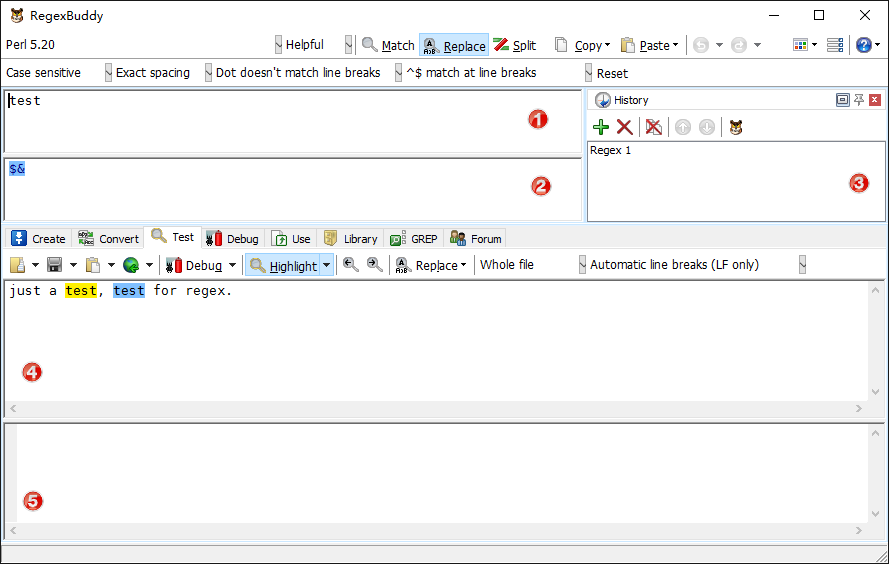
\includegraphics[width=18cm]{FIG/regexbuddy.png}
  \caption{RegexBuddy界面}
  \label{fig:regexbuddy}
\end{figure}
\clearpage{}

\begin{description}
\item[JGsoft PowerGREP] \hfill \\
  PowerGREP RegexBuddy的兄弟软件,同是JGsoft开发,是grep在Windows平台的实现和增强。
\item[Debuggex] \hfill \\
  https://www.debuggex.com/
\item[grep] \hfill \\
  grep
\item[UltraEdit, Notepad++] \hfill \\
  UltraEdit, Notepad++
\item[Vim] \hfill \\
  编辑器之神Vim
\end{description}

\clearpage{}
\begin{description}
\item[\textcolor{red}{GNU Emacs}] \hfill \\
  GNU Emacs中正则表达式异常强大,除了基本的 正向正则查找\keys{C-M-s}、反向正则查找\keys{C-M-r}、正则替换\texttt{M-x replace-regexp}、查询式正则替换\texttt{M-x query-replace-regexp}、保留行\texttt{M-x keep-lines}、删除行\texttt{M-x flush-lines}、\ldots 等等,Emacs正则表达式替换时还能直接执行 LISP\footnote{出生自1958年,但目前仍很活跃的一门编程语言,尤其在AI领域中。} Form\footnote{简言之:可以直接执行LISP代码,利用强大的编程语言提供的函数方法去处理文本。}。详见\ref{sec:emacs}。
\end{description}
\begin{figure}[htbp]
  \centering
  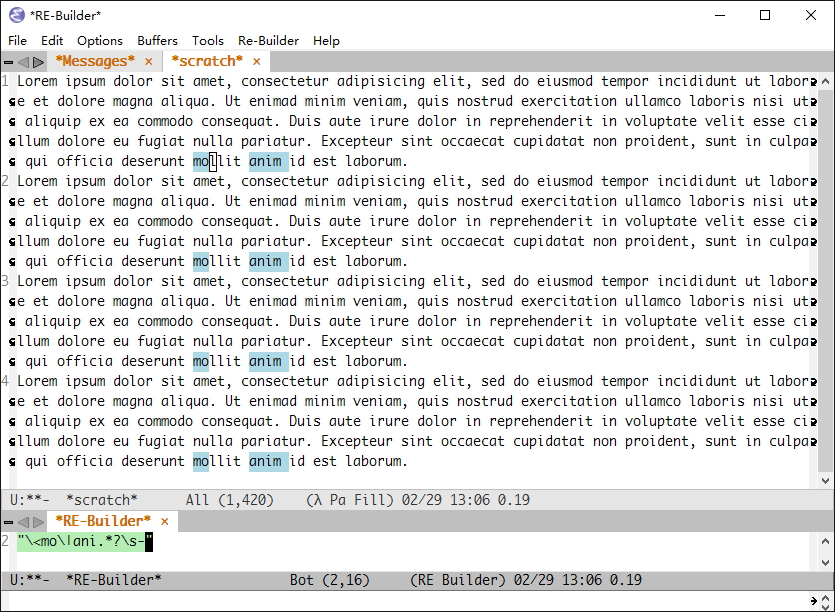
\includegraphics[width=15cm]{FIG/emacs-re-builder.png}
  \caption{GNU Emacs中RE-Builder模式}
  \label{fig:emacs-re-builder}
\end{figure}

\begin{description}
\item[sed \& awk] \hfill \\
  sed and awk
\end{description}

\clearpage{}

\subsection[应用案例]{应用案例 \textcolor{lightgray}{\textsc{Application Cases}}}
\label{sec:cases}

\subsubsection{Perl正则表达式王国}
\label{sec:perl}



%\begin{lstlisting}[language=perl]
%
%\end{lstlisting}

\subsubsection{Python}
\label{sec:python}

Python

\subsubsection{PHP PCRE}
\label{sec:php-pcre}

PHP中使用PCRE\footnote{PCRE, Perl Compatible Regular Expressions} \par

\subsubsection{sed \& awk}
\label{sec:sed-awk}

sed \par

awk \par

\subsubsection{grep}
\label{sec:grep}

grep, egrep, fgrep \par

\subsubsection{Swift}
\label{sec:swift}

Apple Swift

\subsubsection{Java}
\label{sec:java}

\subsubsection{.NET Framework 正则表达式}
\label{sec:dotnet-regex}

\href{https://msdn.microsoft.com/zh-cn/library/az24scfc.aspx}{.NET Framework 正则表达式}


\subsubsection{JavaScript}
\label{sec:javascript}

\subsubsection{Adobe Dreamweaver 表格处理}
\label{sec:adobe-dw}

\subsubsection{VBA中使用正则表达式}
\label{sec:vba}
VBA\footnote{Visual Basic for Application,Microsoft Office套件宏语言。}是不直接支持正则表达式的,需要借助 VBScript RegExp Object,具体请参考\href{http://msdn.microsoft.com/en-us/library/ms974570.aspx}{Microsoft Beefs Up VBScript with Regular Expressions}。
\begin{lstlisting}[language=VBScript]
Sub IndentParaWithRegEx()
' PowerPoint VBA 批量给指定字符开头段落加动画
Dim oSld As Slide
Dim oShp As Shape
Dim i As Integer
' 正则相关变量
Dim regx As Object, oMatch As Object
strPattern = "^开头字符串"

Set regx = CreateObject("vbscript.regexp")
With regx
    .Global = True
    .IgnoreCase = True
    .Pattern = strPattern
End With
    
For Each oSld In ActivePresentation.Slides
    For Each oShp In oSld.Shapes
        If oShp.HasTextFrame Then
            If oShp.TextFrame2.HasText Then
                With oShp.TextFrame2.TextRange
                    For i = 1 To .Paragraphs.Count
                        With .Paragraphs(i)
                             ' 可能会出现多个匹配项的
                            If (regx.Test(.Text) = True) Then
                                .ParagraphFormat.FirstLineIndent = 0
                            End If
                        End With
                    Next i 'para
                End With
            End If 'has text
        End If 'has textframe
    Next oShp
Next oSld
End Sub  
\end{lstlisting}

\subsubsection{GREP for Adobe InDesign}
\label{sec:indesign}

\subsubsection{神的编辑器GNU Emacs之正则神器}
\label{sec:emacs}

\section{后记}
\label{sec:postscript}

后记 \par


\end{document}

%%% Local Variables:
%%% mode: latex
%%% TeX-master: t
%%% End:
